%knob: piqué sur internet: https://tex.stackexchange.com/questions/525535/creating-a-audio-volume-dial-using-tikz
\def\centerarc[#1](#2)(#3:#4:#5)
              { \draw[#1] ($(#2)+({#5*cos(#3)},{#5*sin(#3)})$) arc (#3:#4:#5); }


\newcommand\knob[1]{
\centerarc[name path=arcc,fill=none,draw=black,line width=0.2]($(#1)$)(-60:240:2mm)
%\foreach \t [count=\i from 0] in {-60,-30,...,240}{
\foreach \t [count=\i from 0] in {240,210,...,-60}{
\path [name path=\t]($(#1)$)--++(\t:8.2mm);
\path [name intersections={of=arcc and \t,by={\t1}}];
\draw [line cap=round, line width=0.2](\t1)--++(\t:0.5mm);
\path (\t1)--++(\t:1.5mm)node{\scalebox{0.5}{$\i$}};
}
}

\begin{tikzpicture}[>=stealth']
  \node[draw=black,minimum height=1cm] (arm) {ARM};
  \node[draw=black, below of=arm,minimum width=1.5cm, yshift=-0.4cm] (ip) {Faust IP};
  \node[draw=black,left of=arm, xshift=-0.5cm,rounded rectangle](type){\tiny HW/SW ?};
  \node[draw=black, fit=(arm)(ip)(type),minimum height=1.5cm,minimum width=1.5cm][thick] (zybo) {};

  \node[draw=black,yshift=1cm,xshift=-0.5cm,minimum width=2.5cm,minimum height=1cm,left=of zybo,label={[xshift=-0.5cm,yshift=-0.1cm]\tiny Controller Board}] (interfBoard) {};
  \knob{$(interfBoard)+(-0.5cm,0cm)$};
  \knob{$(interfBoard)+(0.5cm,0cm)$};
  \node[draw=black,inner sep=0pt,minimum width=2.5cm,minimum height=1.5cm,below of=interfBoard,  yshift=-0.7cm,label={[xshift=-0.8cm,yshift=-0.1cm]\tiny Host PC}] (hostPC) {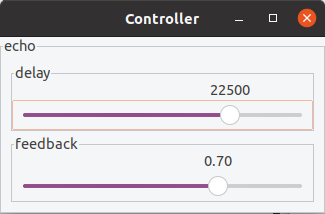
\includegraphics[width=2.5cm]{gtkUI.png}};
  
  \node[right of=hostPC,yshift=0.15cm,xshift=1cm] (uart) {\tiny UART/USB};
  \node[right of=interfBoard,yshift=0.15cm,xshift=0.6cm] (spi) {\tiny SPI};


 \draw[<-][thick] (ip) -- node[right]{\footnotesize s-AXI} (arm);
 \draw[->][thick] (type) -- (arm);
 \draw[->][thick] (hostPC) --++(100pt,0pt) --++(0pt,30pt);
 \draw[->][thick] (interfBoard) --++(100pt,0pt) --++(0pt,-6pt);

\end{tikzpicture}

